\documentclass[dvipdfmx]{standalone}

\usepackage{amssymb, amsmath}
\usepackage{tikz}

\usetikzlibrary{bayesnet}

\begin{document}

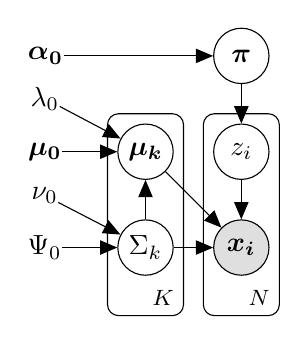
\begin{tikzpicture}[x=0.5cm,y=0.5cm]

  \node[obs] (x_i){$\boldsymbol{x_i}$};

  \node[latent, above=of x_i] (z_i){$z_i$};
  \node[latent, above=of z_i] (pi){$\boldsymbol{\pi}$};
  \node[latent, left=of z_i] (mu_k){$\boldsymbol{\mu_k}$};
  \node[latent, left=of x_i] (sigma_k){$\Sigma_k$};

  \node[const, left=0.7 cm of sigma_k] (Psi_0){$\Psi_0$};
  \node[const, above=0.4cm of Psi_0] (nu_0){$\nu_0$};

  \node[const, left=0.7 cm of mu_k] (mu_0){$\boldsymbol{\mu_0}$};
  \node[const, above=0.4cm of mu_0] (lambda_0){$\lambda_0$};

  \node[const, left=1.9cm of pi] (alpha_0){$\boldsymbol{\alpha_0}$};

  \edge{alpha_0}{pi};
  \edge{lambda_0}{mu_k};
  \edge{mu_0}{mu_k};
  \edge{nu_0}{sigma_k};
  \edge{Psi_0}{sigma_k};
  \edge{pi}{z_i};
  \edge{z_i}{x_i};
  \edge{mu_k}{x_i};
  \edge{sigma_k}{x_i};
  \edge{sigma_k}{mu_k};

  \plate{N}{(z_i)(x_i)}{$N$};
  \plate{K}{(mu_k)(sigma_k)}{$K$};

\end{tikzpicture}

\end{document}
